% Compile either presentation.tex or presentation-handout.tex

\setbeamertemplate{footline}[frame number]  % include frame numbers
\usefonttheme[onlymath]{serif}  % use "article"-style math font

\usepackage[utf8]{inputenc} % allow utf-8 input
%\usepackage[T1]{fontenc}    % use 8-bit T1 fonts
\usepackage{hyperref}       % hyperlinks
\usepackage{url}            % simple URL typesetting
\usepackage{booktabs}       % professional-quality tables
\usepackage{amsmath}
\usepackage{amssymb}
\usepackage{amsthm}
\usepackage{amsfonts}       % blackboard math symbols
\usepackage{mathtools}
\usepackage{nicefrac}       % compact symbols for 1/2, etc.
\usepackage{microtype}      % microtypography
\usepackage{algorithm}
\usepackage{algpseudocode}
\usepackage{graphicx}
\usepackage{outlines}
\usepackage{dsfont}
\usepackage{float}
\usepackage{caption}
\usepackage{tikz}
\usepackage{multirow}
\usepackage{bigdelim}
\usepackage{scalerel}

\usetikzlibrary{bayesnet,positioning}

\newcommand{\nth}{^{\text{th}}}
\newcommand{\len}{\mathop{\text{len}}}
\newcommand{\indicator}{\mathds{1}}
\newcommand{\hackystatei}[1]{\State \parbox[t]{\dimexpr\linewidth-\algorithmicindent}{#1\strut}}
\newcommand{\hackystateii}[1]{\State \parbox[t]{\dimexpr\linewidth-\algorithmicindent-\algorithmicindent}{#1\strut}}

\newcommand{\customSectionFrame}[1]{%
  \begin{frame}[c]{ } %
  \Large
  \color[rgb]{0,0,0.6}
  \centering %
  #1 %
  \end{frame}%
  }

\setbeamertemplate{blocks}[default]
\setbeamertemplate{navigation symbols}{}  % Omit navigation buttons
\setbeamertemplate{bibliography item}{\insertbiblabel}

\begin{document}

\begin{frame}
\vspace{3em}
\begin{center}
\structure{\Large{Hierarchical Topic Models}} \\[1em]
Andrew Leverentz \\[1em]
{ \small
\emph{Research Examination, Fall Quarter 2017} \\
\emph{UC San Diego, Dept.\ of Computer Science and Engineering}} \\[2em]
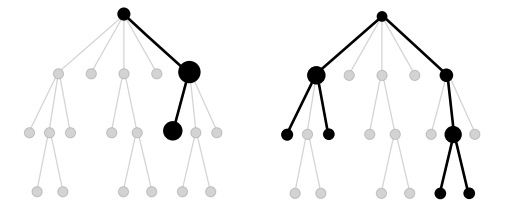
\includegraphics[width=0.7\textwidth]{../figures/title_image.png} \\[1em]
{\color[rgb]{0.5,0.5,0.5} \tiny Image Source: Paisley et al \cite{paisley2015nhdp}}
\end{center}
\end{frame}

\begin{frame}
\frametitle{Context}
\begin{itemize}[<+->]
\item Internet and digital archives $\rightarrow$ large collections of text data
\item How can we navigate these collections efficiently?
\item Typical task: find sets of documents that share the same topic or subject matter
\item Ambiguities of natural language $\rightarrow$ superficial attributes of documents aren't enough
    \begin{itemize}[<+->]
    \item \emph{Synonymy}: Many words, same meaning
    \item \emph{Polysemy}: One word, many meanings (depending on context)
    \end{itemize}
\item We need a notion of \emph{latent semantics}, or underlying meaning
\end{itemize}
\end{frame}

\begin{frame}
\frametitle{Goals}
\begin{itemize}[<+->]
\item General approach: documents are mixtures of topics, which are distributions over the vocabulary
\item Probability provides a natural framework for this
\item Topics can exist at different levels of abstraction (e.g., \emph{baseball} and \emph{basketball} are distinct subtopics under \emph{sports})
\item Can we learn a hierarchy of topics based on a particular corpus?
\item Similar to the Dewey Decimal System or Library of Congress Classification
\end{itemize}
\end{frame}

\begin{frame}
\frametitle{Example: Documents as Mixtures of Topics}
\begin{tabular}{rrll}
Topics:
&$\theta_1$ &$=$ ``sports'' &
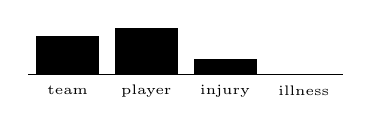
\begin{tikzpicture}[baseline=0.2cm]
\draw (0,0) -- (4,0);
\fill (0.1, 0) rectangle (0.9, 0.5);
\fill (1.1, 0) rectangle (1.9, 0.6);
\fill (2.1, 0) rectangle (2.9, 0.2);
\node at (0.5, -0.2) {\tiny team};
\node at (1.5, -0.2) {\tiny player};
\node at (2.5, -0.2) {\tiny injury};
\node at (3.5, -0.2) {\tiny illness};
\end{tikzpicture}
\\
&$\theta_2$ &$=$ ``medicine'' &
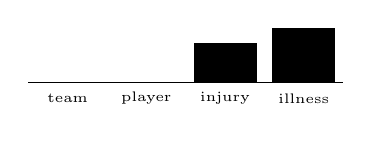
\begin{tikzpicture}[baseline=0.2cm]
\draw (0,0) -- (4cm,0);
\fill (2.1, 0) rectangle (2.9, 0.5);
\fill (3.1, 0) rectangle (3.9, 0.7);
\node at (0.5, -0.2) {\tiny team};
\node at (1.5, -0.2) {\tiny player};
\node at (2.5, -0.2) {\tiny injury};
\node at (3.5, -0.2) {\tiny illness};
\end{tikzpicture}
\\[3em]
%
Documents:
&$\phi_1$ &$=$ ``document 1'' &

\begin{tikzpicture}[baseline=0.2cm]
\draw (0,0) -- (4,0);
\fill (0.2, 0) rectangle (1.8, 0.7);
\fill (2.2, 0) rectangle (3.8, 0.3);
\node at (1, -0.2) {\tiny topic 1};
\node at (3, -0.2) {\tiny topic 2};
\end{tikzpicture}
\\
&$\phi_2$ &$=$ ``document 2'' &

\begin{tikzpicture}[baseline=0.2cm]
\draw (0,0) -- (4,0);
\fill (0.2, 0) rectangle (1.8, 0.3);
\fill (2.2, 0) rectangle (3.8, 0.7);
\node at (1, -0.2) {\tiny topic 1};
\node at (3, -0.2) {\tiny topic 2};
\end{tikzpicture}
\end{tabular}
\end{frame}

\begin{frame}
\frametitle{Outline}
\begin{itemize}[<+->]
\item ``Flat'' topic models
\item Bayesian inference algorithms
\item Learning hierarchies of topics
\end{itemize}
\end{frame}

%%%%%%%%%%%%%

\customSectionFrame{``Flat'' Topic Models}

\begin{frame}
\frametitle{Latent Semantic Analysis: A Non-Probabilistic Precursor}
\begin{itemize}[<+->]
\item Compute matrix of word frequencies:
\[ M_{i,j} = \text{number of times the $i\nth$ word appears in document $j$} \]
\item Optionally, transform via per-term and per-document statistics
\[ X_{i,j} = f(M_{i,j}, M_{i,1:D}, M_{1:N,j}) \]
\item Compute singular-value decomposition (SVD) of this matrix
\[ X = U \Sigma V^\top \]
\item Low-rank truncation represents documents and terms as low-dimensional \emph{latent semantic vectors}
\item Similarity between documents $=$ normalized dot product of latent semantic vectors
\end{itemize}
\end{frame}

\begin{frame}
\frametitle{Probabilistic Latent Semantic Analysis}
\begin{itemize}[<+->]
\item Idea: frequencies of words in documents determined by probabilities
\item There are $K$ latent topics, and each $\theta_k$ is a distribution over words in the vocabulary
\item For document $d$, the vector $\phi_d$ is a distribution over topics
\item For the $n\nth$ word in document $d$:
\begin{alignat*}{2}
\text{Select a topic:}&\qquad& z_{d,n} &\sim \text{Categorical}(\phi_d) \\
\text{Select a word:}&\qquad& t_{d,n} &\sim \text{Categorical}(\theta_{z_{d,n}})
\end{alignat*}
\onslide<.->
\begin{center}
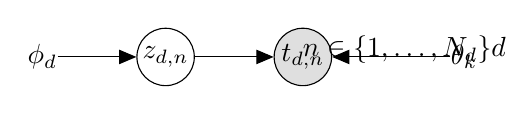
\begin{tikzpicture}
\node[obs] (t) {$t_{d,n}$};
\node[const, right=1.5cm of t] (theta) {$\theta_k$};
\node[latent, left=of t] (z) {$z_{d,n}$};
\node[const, left=of z] (phi) {$\phi_d$};

\edge{phi}{z};
\edge{theta}{t};
\edge{z}{t};

\centeredPlate{word-plate}{(t)(z)}{$n \in \{1, \ldots, N_d\}$};
\centeredPlate{doc-plate}{(word-plate)(phi)}{$d \in \{1, \ldots, D\}$};
\centeredPlate{topic-plate}{(theta)}{$k \in \{1, \ldots, K\}$};
\end{tikzpicture}
\end{center}
\end{itemize}

\begin{itemize}[<+->]
\item Infer values of $\theta_k$, $\phi_d$ using maximum likelihood
\end{itemize}
\end{frame}

\begin{frame}
\frametitle{Latent Dirichlet Allocation}
\begin{itemize}[<+->]
\item Extension to PLSA: assume topic mixtures $\phi_d$ and topic vectors $\theta_k$ are drawn from Dirichlet distributions
\item Dirichlet is a distribution over discrete probability distributions; density over simplex:
\[ \text{Dirichlet}(\vec x \mid \vec \alpha) \propto \prod_{k=1}^{\len(\vec\alpha)} x_i^{\alpha_i - 1} \]
\item Dirichlet distribution acts as a \emph{regularizer}, reduces overfitting
\item Allows Bayesian posterior inference
\end{itemize}
\end{frame}

\begin{frame}
\frametitle{Latent Dirichlet Allocation: The Model}
\begin{alignat*}{2}
\theta_k &\sim \text{Dirichlet}(\alpha) &\qquad&\text{for each topic $k$} \\
\phi_d &\sim \text{Dirichlet}(\beta) &\qquad&\text{for each document $d$} \\
z_{d,n} &\sim \text{Categorical}(\phi_d) &\qquad&\text{for the $n\nth$ word in document $d$} \\
t_{d,n} &\sim \text{Categorical}(\theta_{z_{d,n}}) &\qquad&\text{for the $n\nth$ word in document $d$}
\end{alignat*}

\begin{center}
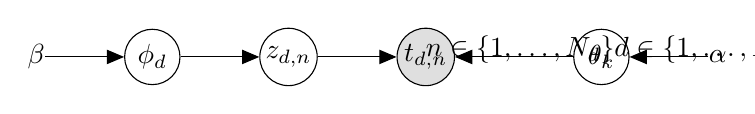
\begin{tikzpicture}
\node[obs] (t) {$t_{d,n}$};
\node[latent, right=1.5cm of t] (theta) {$\theta_k$};
\node[latent, left=of t] (z) {$z_{d,n}$};
\node[latent, left=of z] (phi) {$\phi_d$};
\node[const, right=of theta] (alpha) {$\alpha$};
\node[const, left=of phi] (beta) {$\beta$};

\edge{alpha}{theta};
\edge{phi}{z};
\edge{beta}{phi};
\edge{theta}{t};
\edge{z}{t};

\centeredPlate{word-plate}{(t)(z)}{$n \in \{1, \ldots, N_d\}$};
\centeredPlate{doc-plate}{(word-plate)(phi)}{$d \in \{1, \ldots, D\}$};
\centeredPlate{topic-plate}{(theta)}{$k \in \{1, \ldots, K\}$};
\end{tikzpicture}
\end{center}
\end{frame}

%%%%%%%%%%%%%

\customSectionFrame{Bayesian Inference Algorithms}

\begin{frame}
\frametitle{Posterior Inference}
\begin{itemize}[<+->]
\item Latent-variable models contain \emph{observed} and \emph{latent} random variables
\item Model specifies:
    \begin{itemize}
    \item<.-> \emph{Likelihood}: $p(\text{data} \mid \text{latent variables}, \text{fixed parameters})$
    \item<+-> \emph{Prior}: $p(\text{latent variables} \mid \text{fixed parameters})$
    \end{itemize}
\item Goal: try to estimate the \emph{posterior} via Bayes' rule
\begin{align*}
\MoveEqLeft
p(\text{latent variables} \mid \text{data}, \text{fixed parameters}) \\
&=
\frac{\text{Likelihood} \times \text{Prior}}
     {p(\text{data} \mid \text{fixed parameters})}
\end{align*}
\item Denominator: marginalization is often intractable
\item Need approximate inference methods
\end{itemize}
\end{frame}

\begin{frame}
\frametitle{Gibbs Sampling}
\begin{itemize}[<+->]
\item Markov Chain Monte Carlo (MCMC) method
    \begin{itemize}[<+->]
    \item \emph{Monte Carlo}: Estimate a quantity by drawing samples from a random distribution
    \item \emph{Markov Chain}: Find stationary distribution of a stochastic process where update rules depend only on previous state
    \end{itemize}
\item State vector $\vec z$; each component corresponds to a latent variable
\item Repeatedly update $\vec z$ by iterating through latent variables, updating $z_k$ by sampling from its \emph{complete conditional}:
\[ p(z_k \mid \vec z_{-k}, \vec x) \]
Here, $\vec z_{-k}$ denotes all components of $\vec z$ except $z_k$
\item The distribution of the samples $\vec z$ approaches the true posterior $p(\vec z \mid \vec x)$
\end{itemize}
\end{frame}

\begin{frame}
\frametitle{Collapsed Gibbs Sampling}
\begin{itemize}[<+->]
\item For some models, we can eliminate some latent variables by marginalization
\item For the remaining latent variables, we compute a modified form of the complete conditionas:
\[ p(z_k \mid \vec z_{\text{subset}-k}, \vec x) \]
\item Running Gibbs sampling based on these distributions yields an estimate for
\[ p(\vec z_{\text{subset}} \mid \vec x) \]
%\item Estimating the eliminated variables requires post-processing
\end{itemize}
\end{frame}

\begin{frame}
\frametitle{Variational Inference}
\begin{itemize}[<+->]
\item Approximation technique: select an approximating family of distributions and search for best approximation
\item Measure closeness using reversed Kullback-Leibler divergence
\item Mean-field approximation: consider parameterized functions which factor cleanly:
\[ q(\vec z) = \prod_k q_k(z_k; \nu_k) \]
\item Minimizing reversed KL corresponds to maximizing \emph{evidence lower bound} (ELBO):
\[ \text{ELBO} = E_q[\log p(\vec z, \vec x)] - E_q[\log q(\vec z)] \]
\end{itemize}
\end{frame}

\begin{frame}
\frametitle{Coordinate-Ascent Variational Inference}
\begin{itemize}[<+->]
\item Coordinate ascent: optimize one latent variable's parameters at a time
\item Works best for exponential-family models, where conditional distributions can be written as
\[ p(x \mid \theta) = h(x) \exp( \alert<.(1)| handout:0>{\eta(\theta)} \cdot \alert<.(2)| handout:0>{T(x)} - a(\theta)) \]
\onslide<+->{(\alert<.| handout:0>{$\eta(\theta) =$ \emph{natural parameters}}, \alert<+| handout:0>{$T(x) =$ \emph{sufficient statistics}})} \pause
\item For exponential-family models, the update rule for $z_k$ is
\[ \nu_k = E_q[\eta_k(\vec z_{-k}, \vec x)] \]
where $\eta_k$ denotes the natural parameters of the complete conditional of $z_k$
\end{itemize}
\end{frame}

\begin{frame}
\frametitle{Stochastic Variational Inference: Context}
\begin{itemize}[<+->]
\item Generic model with local (per-observation) and global variables:
\begin{center}
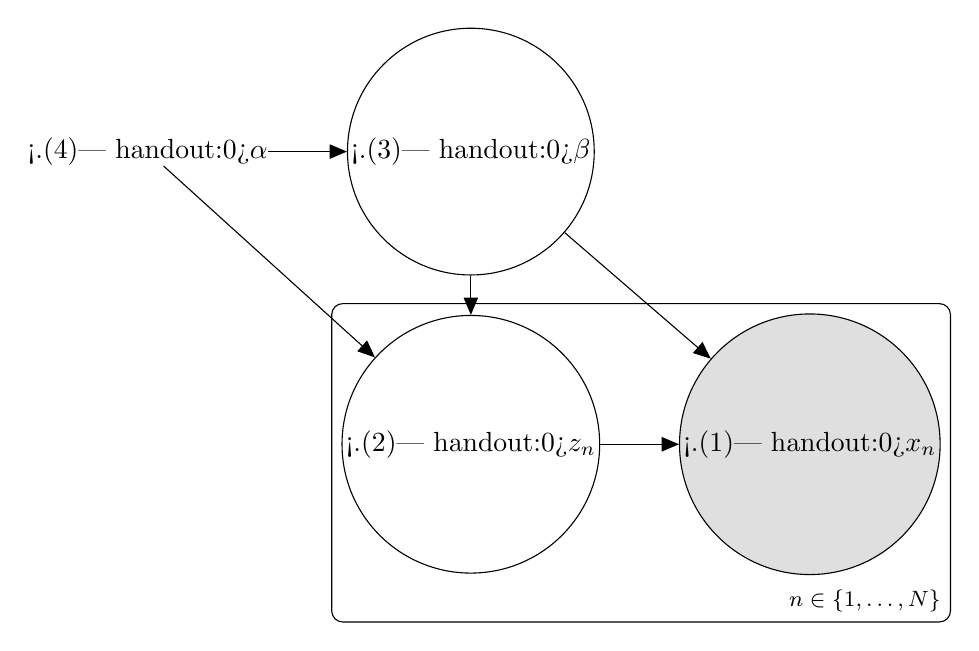
\begin{tikzpicture}
\node[obs] (x) {\alert<.(1)| handout:0>{$x_n$}};
\node[latent, left=of x] (z) {\alert<.(2)| handout:0>{$z_n$}};
\node[latent, above=0.5cm of z] (beta) {\alert<.(3)| handout:0>{$\beta$}};
\node[const, left=of beta] (alpha) {\alert<.(4)| handout:0>{$\alpha$}};

\edge{z}{x};
\edge{beta}{z};
\edge{beta}{x};
\edge{alpha}{beta};
\edge{alpha}{z};

\plate{obs-plat}{(x)(z)}{$n \in \{1, \ldots, N\}$};
\end{tikzpicture}
\end{center}
\onslide<+->{\alert<.| handout:0>{$x_n$}: observed data} \\
\onslide<+->{\alert<.| handout:0>{$z_n$}: local variables (one per observation)} \\
\onslide<+->{\alert<.| handout:0>{$\beta$}: global variable (shared for all observations)} \\
\onslide<+->{\alert<.| handout:0>{$\alpha$}: fixed parameters}
\item Complete conditional for local variables simplifies:
\[ p(z_n \mid \alpha, \beta, z_{-n}, x_{1:N}) = p(z_n \mid \alpha, \beta, x_n) \]
\item Complete conditional for global variable requires full dataset:
\[ p(\beta \mid \alpha, z_{1:N}, x_{1:N}) \]
\end{itemize}
\end{frame}

\begin{frame}
\frametitle{Stochastic Variational Inference: Natural Gradient}
\begin{itemize}[<+->]
\item Euclidean distance on variational parameters may not reflect ``true'' distance between distributions
\item Rather than standard gradient of the objective function ($\nabla \mathcal L$), use natural gradient $G^{-1} \nabla \mathcal L$
\item $G$ is a matrix (\emph{metric tensor}) that encodes local information about ``true'' distances
\item With a symmetric version of KL divergence and a model with exponential-family distributions, $G$ cancels cleanly:
\[ G^{-1} \nabla \mathcal L = E_q[\eta] - \nu \]
where $\nu$ is the current value of the local variational params
\item For local variables, the update rule is the same as in CAVI:
\[ \nu^{\text{local}} = E_q[\eta^{\text{local}}] \]
\end{itemize}
\end{frame}

\begin{frame}
\frametitle{Stochastic Variational Inference: Global Updates}
\begin{itemize}[<+->]
\item For global variables, repeatedly draw \emph{mini-batches} $b$ containing $S$ observations
\item Compute an \emph{unbiased estimate} of the natural gradient $G^{-1} \nabla \mathcal L$ for each batch:
\[ \mu = E_q[\alert<.(1)| handout:0>{\eta^{\text{global}}_b}] - \nu^{\text{global}} \]
\onslide<+->{Here, \alert<.| handout:0>{$\eta^{\text{global}}_b$} denotes the natural parameters of the complete conditional of the global variable, but with the true dataset replaced by $N / S$ copies of the mini-batch $b$}
\item Update according to a decaying schedule of step sizes $\rho_t$:
\begin{align*}
\nu^{\text{global}}
&\gets \nu^{\text{global}} + \rho_t \, \mu \\
\onslide<+->{ &= (1-{\rho_t}) \nu^{\text{global}} + {\rho_t} \, E_q[\eta^{\text{global}}_b] }
\end{align*}
%\onslide<+->{Here, \alert<.>{$\rho_t$} should satisfy $\sum_{t\geq1} \rho_t = \infty$ and $\sum_{t\geq1} \rho_t^2 < \infty$}
\end{itemize}
\end{frame}

%%%%%%%%%%%%%

\customSectionFrame{Learning Topic Hierarchies}

\begin{frame}
\frametitle{Topic Modeling with Hierarchies}
\begin{itemize}[<+->]
\item Goal: extend LDA model so that: %\alt<.>{\ldots}{:}
    \begin{itemize}[<+->]
    \item Topics are arranged in a tree \\ (root $\rightarrow$ abstract; leaves $\rightarrow$ concrete)
    \item The size and structure of the tree can be determined in a data-driven way
    \end{itemize}
\item Documents can combine topics, but in a more constrained way
    \begin{itemize}
    \item If a document draws words from one node, then it should also be somewhat likely to draw words from ancestor nodes
    \end{itemize}
\item We'll discuss two main models:
    \begin{itemize}
    \item Nested Chinese Restaurant Process
    \item Nested Hierarchical Dirichlet Process
    \end{itemize}
\end{itemize}
\end{frame}

\begin{frame}
\frametitle{Nested Chinese Restaurant Process}
\begin{itemize}[<+->]
\item Idea: Each document samples a path from an infinite tree
\item Within each document, we can only select nodes (ie, topics) from the sampled path
\vspace{1em}
\item How to define distributions over paths in an infinite (or arbitrarily large) tree? \\
\onslide<+->{Nested Chinese Restaurant Process}
\item How to define distributions over arbitrarily large partitions? \\
\onslide<+->{Chinese Restaurant Process}
\end{itemize}
\end{frame}

\begin{frame}
\frametitle{Chinese Restaurant Process: Distribution Over Partitions}
\begin{itemize}[<+->]
\item Analogy: Sequence of customers entering a restaurant
\item Infinitely many tables, each with infinite capacity
\item First customer always sits at first table
\item When $n \geq 1$ customers have been seated, the next customer follows these rules:
    \begin{itemize}
    \item If the first $k$ tables are occupied, with the $i\nth$ table containing $m_i$ customers, sit at table $i$ with probability $\frac{m_i}{n+\alpha}$
    \item Sit at the next empty table with probability $\frac{\alpha}{n + \alpha}$
    \end{itemize}
\item Parameter $\alpha$: As $\alpha \to \infty$, number of occupied tables increases
\item Stick-breaking construction:
    \begin{itemize}
    \item Draw infinite sequence of beta-distributed variables:
    \[ V_k \sim \text{Beta}(1, \alpha) \qquad \text{for $k \geq 1$} \]
    \item Draw table index $k$ with probability $\pi_k = V_k \prod_{j=1}^{k-1} (1-V_j)$
    \end{itemize}
\end{itemize}
\end{frame}

\begin{frame}
\frametitle{Dirichlet Process: Distribution Over Grouped Data}
\begin{itemize}[<+->]
\item Alternative formulation: when CRP is used as an index into a set of i.i.d.\ random variables
\item Parameterized by $\alpha$ and a base distribution $G_0$
\item Let $X \sim \text{DP}(\alpha, G_0)$ denote:
\begin{align*}
\onslide<+->{\theta_k &\sim G_0} \\
\onslide<+->{V_k &\sim \text{Beta}(1, \alpha)} \\
\onslide<+->{\pi_k &= V_k \prod_{j=1}^{k-1} (1-V_j)} \\
\onslide<+->{X &= \sum_{k \geq 1} \pi_k \delta_{\theta_k}}
\end{align*}
\item So, $X$ is a discrete distribution over a countable set of ``atoms'' drawn from $G_0$
\end{itemize}
\end{frame}

\begin{frame}
\frametitle{Nested CRP: Distribution Over Paths}
\begin{itemize}[<+->]
\item Analogy: Infinitely many restaurants, arranged in a tree
\item Customers enter the ``root'' restaurant and select a table
\item Once seated, customers move to a restaurant indicated by a card at their table
\item This process repeats indefinitely at new restaurants
\end{itemize}
\end{frame}

\begin{frame}
\frametitle{Nested CRP: Distribution Over Paths}
\begin{itemize}[<+->]
\item A single draw from the NCRP is a distribution over infinite paths (finite-depth variant also exists)
\item Stick-breaking construction:  $T \sim \text{NCRP}(\alpha)$ denotes:
\begin{align*}
\onslide<+->{V_r &\sim \text{Beta}(1, \alpha) \qquad \text{for any finite-length path $r$}} \\
\onslide<+->{V_{()} &= 1} \\
\onslide<+->{\pi_{()} &= 1} \\
\onslide<+->{\pi_{r[1:\ell]} &= \pi_{r[1:\ell-1]} \cdot \left( V_{r[1:\ell]} \prod_{j=1}^{r[\ell]-1} (1-V_{r[1:\ell-1],j}) \right)} \\
\onslide<+->{T &= \sum_{{\mathclap{r : \text{infinite path}}}} \pi_r \delta_r}
\end{align*}
\end{itemize}
\end{frame}

\begin{frame}
\frametitle{The GEM Distribution}
\begin{itemize}[<+->]
\item Within a path, how to sample individual nodes?
\item Select depth via GEM distribution over positive integers \\
(GEM = Griffiths, Engen, and McCloskey)
\item Notation: $\vec \pi \sim \text{GEM}_2(\alpha_1, \alpha_2)$ is shorthand for
\begin{align*}
V_k &\sim \text{Beta}(\alpha_1, \alpha_2) \qquad \text{for } k \geq 1 \\
\pi_k &= V_k \prod_{j=1}^{k-1} (1-V_j) \qquad \text{for } k \geq 1
\end{align*}
\item Then, select depth via
\begin{align*}
Z &\sim \text{Categorical}(\{\pi_k\}_{k \geq 1})
\end{align*}
\end{itemize}
\end{frame}

\begin{frame}
\frametitle{NCRP Topic Model}
\begin{itemize}[<+->]
\item Draw an infinite tree of topics, $\theta_r \sim \text{Dirichlet}(\alpha^{(\theta)})$
\item Draw a global distribution over paths, $T \sim \text{NCRP}(\alpha^{(V)})$
\item For each document $d$:
    \begin{itemize}
    \item Draw a path $c_d \sim T$
    \item Draw a distribution over depths $\phi_d \sim \text{GEM}_2(\alpha^{(\phi)}_1, \alpha^{(\phi)}_2)$
    \item For each word-slot $n$:
        \begin{itemize}
        \item Draw a depth $z_{d,n} \sim \text{Categorical}(\phi_d)$
        \item Draw a vocabulary word $t_{d,n} \sim \text{Categorical}(\theta[c_d[1:z_{d,n}]])$
        \end{itemize}
    \end{itemize}
\end{itemize}
\end{frame}

\begin{frame}
\frametitle{NCRP Topic Model}
\begin{center}
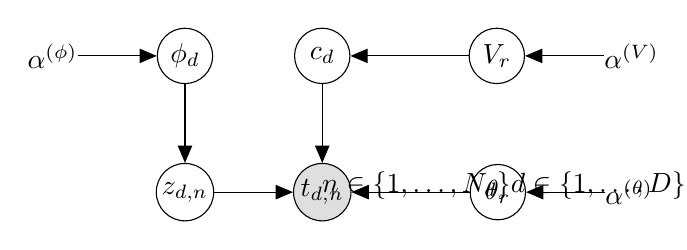
\begin{tikzpicture}
\node[obs] (t) {$t_{d,n}$};
\node[latent, above=of t] (c) {$c_d$};
\node[latent, right=1.5cm of c] (v) {$V_r$};
\node[latent, right=1.5cm of t] (th) {$\theta_r$};
\node[latent, left=of t] (z) {$z_{d,n}$};
\node[latent, above=of z] (phi) {$\phi_d$};
\node[const, left=of phi] (alphaPhi) {$\alpha^{(\phi)}$};
\node[const, right=of v] (alphaV) {$\alpha^{(V)}$};
\node[const, right=of th] (alphaTheta) {$\alpha^{(\theta)}$};

\edge{phi}{z};
\edge{z}{t};
\edge{c}{t};
\edge{v}{c};
\edge{th}{t};
\edge{alphaPhi}{phi};
\edge{alphaV}{v};
\edge{alphaTheta}{th};

\centeredPlate{word-plate}{(t)(z)}{$n \in \{1, \ldots, N_d\}$};
\centeredPlate{doc-plate}{(phi)(c)(z)(t)(word-plate)}{$d \in \{1, \ldots, D\}$};
\centeredPlate{tree-plate}{(th)(v)}{\begin{tabular}{c}$r: $ path to \\ any node\end{tabular}};
\end{tikzpicture}
\end{center}
\end{frame}

\begin{frame}
\frametitle{NCRP Topic Model: Gibbs Sampling}
\begin{itemize}[<+->]
\item Collapsed Gibbs sampling (marginalize out depth proportions $\phi_d$ and topic vectors $\theta_r$)
\item Griffiths et al \cite{griffiths2004hierarchical}: Finite depth, uses order-dependent ``restaurant analogy'' formulation to avoid tracking infinitely many paths; each sampling step may grow or shrink the tree
\item Blei et al \cite{blei2010ncrp}: Uses lazy evaluation; if final layer is ever sampled, then start tracking one extra layer
\end{itemize}
\end{frame}

\begin{frame}
\frametitle{NCRP Topic Model: Variational Inference}
\begin{itemize}[<+->]
\item Infinitely many latent variables: need additional approximations
\item Start with finite-depth, finite-width tree
\item Depth stays constant, but width may change throughout algorithm
\item Outside of the finite truncation, all variational distributions assumed constant
\item Divide infinite set of paths into finitely many equivalence classes
\item If one equivalence class becomes sufficiently likely, add a representative path from it
\end{itemize}
\end{frame}

\begin{frame}
\frametitle{Nested Hierarchical Dirichlet Process}
\begin{itemize}[<+->]
\item Idea: Global probability distribution over nodes, and each document samples a re-weighted version of that distribution
\item Handles ``hybrid'' topics better than NCRP
\begin{center}
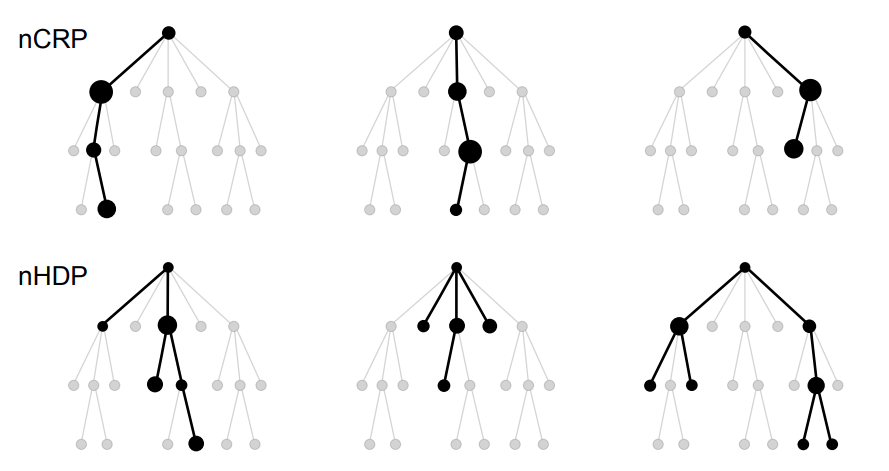
\includegraphics[width=0.8\textwidth]{../figures/ncrp_vs_nhdp.png} \\
\footnotesize Source: Paisley et al \cite{paisley2015nhdp}
\end{center}
\end{itemize}
\end{frame}

\begin{frame}
\frametitle{Hierarchical Dirichlet Process}
\begin{itemize}[<+->]
\item A model for grouped data, with unbounded number of groups
\item Formulation:
\begin{align*}
H &\sim \text{DP}(\alpha, G_0) \\
H_d &\sim \text{DP}(\beta, H) \\
\mu_{d,n} &\sim H_d \\
x_{d,n} &\sim F(\mu_{d,n})
\end{align*}
\item Global distribution $H$ drawn from Dirichlet Process applied to base distribution $G_0$
\item Per-group distributions $H_d$ drawn from another Dirichlet Process applied to $H$
\end{itemize}
\end{frame}

\begin{frame}
\frametitle{NHDP Topic Model}
\begin{itemize}[<+->]
\item Each node in infinite tree associated with a topic vector
\item NHDP uses an instance of HDP at each node in the infinite tree
\item Interleaves per-document path-propagation variables to define a document-specific distribution over nodes
\end{itemize}
\end{frame}

\begin{frame}
\frametitle{NHDP Topic Model: Generative Process}
Global steps:
\begin{itemize}[<+->]
\item For each node $r$ in the infinite tree, draw a topic vector $\theta_r$
\item For each node $r$ and each $j \geq 1$, draw stick-breaking proportion $V^*_{r,j}$
\end{itemize}
\end{frame}

\begin{frame}
\frametitle{NHDP Topic Model: Generative Process}
\onslide<+->{For each document $d$:}
  \begin{itemize}[<+->]
  \item For each node $r$ in the infinite tree:
    \begin{itemize}
    \item For each $j \geq 1$:
      \begin{itemize}
      \item Draw an index $z^d_{r,j} \geq 1$ according to a discrete distribution with probabilities given by $\pi_k = V^*_{r,k} \prod_{i=1}^{k-1} (1-V^*_{r,i})$.
      \item Draw a beta-distributed stick-breaking proportion $V^d_{r,j}$.
      \end{itemize}
    \item Draw a beta-distributed path-propagation random variable $U^d_r$.
    \end{itemize}
  \item For each word-slot $n$ in document $d$:
    \begin{itemize}
    \item Let $r = ()$, the empty path.
    \item Repeat the following steps until a value for $c^d_n$ is chosen:
      \begin{itemize}
      \item Draw a Bernoulli random variable with mean $U^d_r$.
      \item If the outcome is $1$, then set $c^d_n = r$ and break out of this loop; otherwise, continue.
      \item For all $j \geq 1$, let $S_j =$ set of indices $k$ such that $z^d_{r,k} = j$. \\
      Define $\mu_j = \sum_{k \in S_j} V^d_{r,k} \prod_{i=1}^{k-1} (1-V^d_{r,i})$.
      \item Draw an index $\tilde z \geq 1$ from a discrete probability distribution with probabilities given by $\mu_j$ as defined above.
      \item Update $r \gets (r, \tilde z)$.
      \end{itemize}
    \item Draw a vocabulary word $t^d_n$ from $\text{Categorical}(\theta_{c^d_n})$.
    \end{itemize}
  \end{itemize}
\end{frame}

\begin{frame}
\frametitle{NHDP Topic Model: Conditional Distributions}
{
\footnotesize
\begin{align*}
\theta_r &\sim \text{Dirichlet}(\alpha^{(\theta)}) \\
V^*_{r,j} &\sim \text{Beta}(1, \alpha^{(V^*)}) \\
V^d_{r,j} &\sim \text{Beta}(1, \alpha^{(V)}) \\
U^d_r &\sim \text{Beta}(\alpha^{(U)}_1, \alpha^{(U)}_2) \\
z^d_{r,j} &\sim \sum_{k \geq 1} \left( V^*_{r,k} \prod_{i=1}^{k-1} (1-V^*_{r,i}) \right) \delta_k \\
c^d_n &\sim \sum_{r: \text{path}} A(r, V^d, z^d) \, B(r, U^d) \, \delta_r \\
A(r, V^d, z^d) &= \prod_{m=0}^{\len(r)-1} \sum_{k \geq 1} \indicator \left[ z^d_{r[1:m],k} = r[m+1] \right] \left( V^d_{r[1:m],k} \prod_{i=1}^{k-1} \left( 1 - V^d_{r[1:m],i} \right) \right) \\
B(r, U^d) &= U^d_r \prod_{m=0}^{\len(r)-1} \left( 1 - U^d_{r[1:m]} \right) \\
t^d_n &\sim \text{Categorical}(\theta_{c^d_n})
\end{align*}
}
\end{frame}

\begin{frame}
\frametitle{NHDP Topic Model: Plate Diagram}
\begin{center}
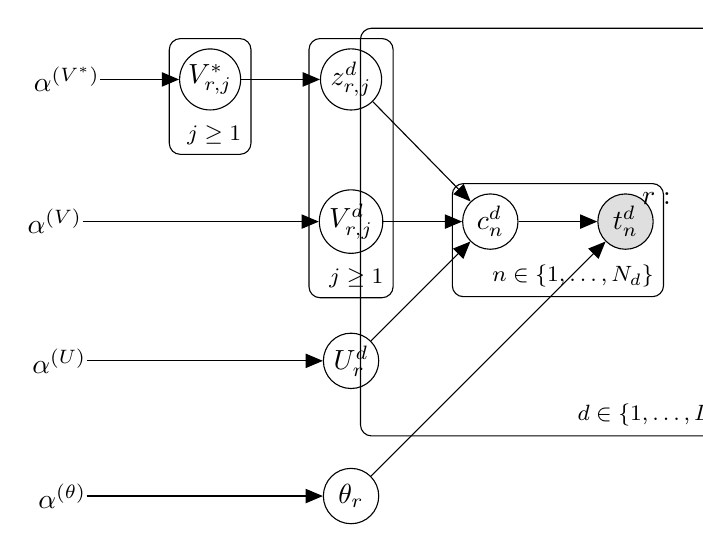
\begin{tikzpicture}
\node[obs] (t) {$t^d_n$};
\node[latent, left=of t] (c) {$c^d_n$};
\node[latent, left=of c] (v) {$V^d_{r,j}$};
\node[latent, below=of v] (u) {$U^d_r$};
\node[latent, above=of v] (z) {$z^d_{r,j}$};
\node[latent, left=of z] (vstar) {$V^*_{r,j}$};
\node[latent, below=of u] (th) {$\theta_r$};
\node[const, left=of vstar] (alphaVstar) {$\alpha^{(V^*)}$};
\node[const, left=3cm of th] (alphaW) {$\alpha^{(\theta)}$};
\node[const, left=3cm of v] (alphaV) {$\alpha^{(V)}$};
\node[const, left=3cm of u] (alphaU) {$\alpha^{(U)}$};
%
\edge{c}{t};
\edge{z}{c}
\edge{v}{c};
\edge{u}{c};
\edge{vstar}{z};
\edge{th}{t};
\edge{alphaV}{v};
\edge{alphaU}{u};
\edge{alphaVstar}{vstar};
\edge{alphaW}{th};
%
\plate{word-plate}{(t)(c)}{$n \in \{1, \ldots, N_d\}$};
\plate{j-plate-1}{(vstar)}{$j \geq 1$};
\plate{j-plate-2}{(z)(v)}{$j \geq 1$};
\centeredPlate{tree-plate}{(u)(th)(j-plate-1)(j-plate-2)}{\begin{tabular}{c}$r: $ path to \\ any node\end{tabular}};
\plate{doc-plate}{(word-plate)(u)(j-plate-2)}{$d \in \{1, \ldots, D\}$};
\end{tikzpicture}
\end{center}
\end{frame}

\begin{frame}
\frametitle{NHDP: Stochastic Variational Inference}
\begin{itemize}[<+->]
\item Use a finite-depth, finite-width tree
\item Simplifications for document-specific indices $z^d_{r,j}$:
    \begin{itemize}
    \item Use Dirac-$\delta$ variational distributions
    \item For any $d$ and any $r$, the indices $z^d_{r,j}$ do not repeat
    \item For each document, greedy algorithm selects small number of nodes to include
    \end{itemize}
\item Greedy algorithm: start with root, add a node only if it increases ELBO by some threshold
\item Remainder of algorithm is a standard application of stochastic variational inference
\end{itemize}
\end{frame}

\begin{frame}
\frametitle{Directions for Future Research}
\begin{itemize}[<+->]
\item Scalable algorithms
\item Interpreting models
\item Incorporating human feedback
\item Moving beyond the bag-of-words model
\item Frameworks for Bayesian non-parametric inference
\end{itemize}
\end{frame}

%%%%%%%%%%%%%

\begin{frame}
\frametitle{Acknowledgements}
\begin{itemize}
\item \textbf{Advisor:} Sanjoy Dasgupta
\item \textbf{LANL Mentor:} Kari Sentz
\item \textbf{Research Exam Committee:} \\ Vineet Bafna (chair), Yoav Freund, Julian McAuley
\end{itemize}
\vspace{2em}
\begin{center}
\Large
\color[rgb]{0,0,0.6}
Thank You!
\end{center}
\end{frame}

{
\setbeamertemplate{frametitle continuation}{}
\setbeamerfont{bibliography item}{size=\tiny}
\setbeamerfont{bibliography entry author}{size=\tiny}
\setbeamerfont{bibliography entry title}{size=\tiny}
\setbeamerfont{bibliography entry location}{size=\tiny}
\setbeamerfont{bibliography entry note}{size=\tiny}
\begin{frame}[allowframebreaks]
\frametitle{References}
\nocite{*}
%\bibliographystyle{amsalpha}
%\bibliographystyle{plainnat}
\bibliographystyle{plain}
\bibliography{../bibliography}
\end{frame}
}

\end{document}
